\documentclass{article}
\usepackage[utf8]{inputenc}
\usepackage{ragged2e}
\usepackage{geometry}
\usepackage{pdfpages}
\usepackage{biblatex}
\geometry{portrait}

\addbibresource{main.bib}

\title{Scientific Calculator}
\author{Anand Kacha (40047673)}

\begin{document}

\maketitle

\tableofcontents

\clearpage

\section{Introduction}
\justifying
A transcendental number \cite{transcendental} is a real (or complex) number which is not an algebraic number. In other words, it can never solve a non-zero algebraic equation. (For example, if $x$ is a non-unit algebraic number ($x^2 \ne x$, which is similar to $x \ne 0 \ne 1$ ) and $y$ is another algebraic number but irrational number. then $x^y$ is transcendental number). Few examples of transcendental numbers are $\pi$, $e$, $2^{\sqrt{2}}$, etc.
\begin{flushleft}
\justifying
One more example of the transcendental number is the Gelfond's constant \cite{gelfondsconstant} which is $e^{\pi}$. Since the transcendental numbers exhibit the properties of infinite numbers, the value of Gelfond's constant approximated to 10 digits is $23.1406926327$
\end{flushleft}

\subsection{Calculation}
\begin{flushleft}
\justifying
To calculate the value of Gelfond's constant, let's take $k_0 = \frac{1}{\sqrt{2}}$ and $k_{n+1} = \frac{1 - \sqrt{1 - k_n^2}}{1 + \sqrt{1 - k_n^2}}$ where $n$ is a positive number. The sequence generated when calculating $(\frac{4}{k_{n+1}})^{2^{-n}}$ rapidly converges to form the Gelfond's constant ($e^\pi$).
\end{flushleft}

\subsection{Properties}
\begin{flushleft}
\justifying
The value of Gelfond's number is not finite. It does not have any visible pattern. The Gelfond's constant is a proof that the number (or series) produced by the algebraic power of two numbers that exhibit transcendence is also exhibits the properties of transcendence. The Gelfond's constant was introduced in order to solve the Hilbert's seventh problem \cite{hilbertsproblems}. One unique property of the Gelfond's constant is that the value of the Gelfond's constant is exactly the same as volume of all unit balls (spheres) with even dimensions in Eucledian Space. The arithmetic operations such as (multiplications, power, multiplications in power, etc) with appropriate algebraic numbers on Gelfond's constant produces the almost integer numbers.
\end{flushleft}

\subsection{Applications}
\begin{flushleft}
\justifying
It is useful when calculating the other constants that help figure the almost integer numbers (e.g. Ramanujan's constant, $e^{\pi} - \pi$, etc.). It is useful to calculate the volume of n-unit balls \cite{nball} in Euclidean Space. Therefore, it can be used to calculate the region in n-class classification problems where each class has a unit value. 
\end{flushleft}

\section{Interview}

\subsection{Questions}
\justifying
\begin{itemize}
    \item Which field are you working in physics? Are you working in any specialization?
    \item How long have you been involved in this field?
    \item Is it theoretical physics or experimental physics?
    \item Do you use any specific device to perform complex calculations?
    \item What features do you think are missing from the device or software you're using?
    \item Are you familiar with Gelfond's constant?
    \item Are you using or working with this constant in any way?
    \item In future, if you come across an application that requires this constant in your equations, would it be good to have it in a software that you're using?
    \item what kind of interface would you prefer for the software or device you'd like to use for calculations?
    \item Would you rather prefer a simple design that is specific to you or a more generic system?
\end{itemize}

\subsection{Response}
\justifying
I have contacted Shubham Bhagat, a PhD student at Concordia University. We've had a text-based interview session through instant messaging platform. Here are the responses I have gathered from her.

\textbf{Q. Which field are you working in physics? Are you working in any specialization?}

A. My topic is related to both chem and physics. Broadly it is organic semiconductors.
\vspace{0.6em}

\textbf{Q. How long have you been involved in this field?}

A. I am completely new to this field. It's been 10 months. Eariler I was working with inorganic semi-conductor.
\vspace{0.6em}

\textbf{Q. Is it theoretical physics or experimental physics?}

A. Experimental
\vspace{0.6em}

\textbf{Q. Do you use any specific device to perform complex calculations?}

A. Not calculation but you can say data processing like which material property we want to explore, then deciding which characterization technique( or simply which instrument) to use and then interpreting the experimental data obtained from that instrument.
\vspace{0.6em}

\textbf{Q. What features do you think are missing from the device or software you're using?}

A. No. Sometimes we don’t have access to all that specific technique or its not possible to measure the samples right away. Some of the software are paid. I would like them to be freely available
\vspace{0.6em}

\textbf{Q. Are you familiar with Gelfond's constant?}

A. No
\vspace{0.6em}

\textbf{Q. Are you using or working with this constant in any way?}

A. No
\vspace{0.6em}

\textbf{Q. In future, if you come across an application that requires this constant in your equations, would it be good to have it in a software that you're using?}

A. It would be nice if I can do some noble work and if that require using this constant then I would surely love to have it in my software
\vspace{0.6em}

\textbf{Q. what kind of interface would you prefer for the software or device you'd like to use for calculations?}

A. I would prefer online interface where I can decide which parameters I would need and easily access it from anywhere. Sometimes one thing does not fit all, and also I won’t be really sure about the way that instrument would have been programmed to do certain calculations.
\vspace{0.6em}

\textbf{Q. Would you rather prefer a simple design that is specific to you or a more generic system?}

A. A generic one which is easy to modify.

\subsection{Analysis}
\justifying
Shubham Bhagat is a PhD student researching organic semiconductors at Concordia Univeristy. She is relatively new to this field. It has been 10 months since she has switched from Inorganic Semi Conductor. Since she has been working in experimental physics, she has to collect the readings from several experiments and process the data she has collected. She does not use a calculator but she uses a desktop computer to crunch the data and derive the useful calculations. Even though she is not familiar with the Gelfond's constant, she is open to the possibility of working with Gelfond's constant whenever needed. Being experimental physicist, she is more comfortable with the desktop based interface where she can customize it based on the experiments she performs. Even though she prefers to customize the platform, she voted to have as much generic system as possible.

\clearpage
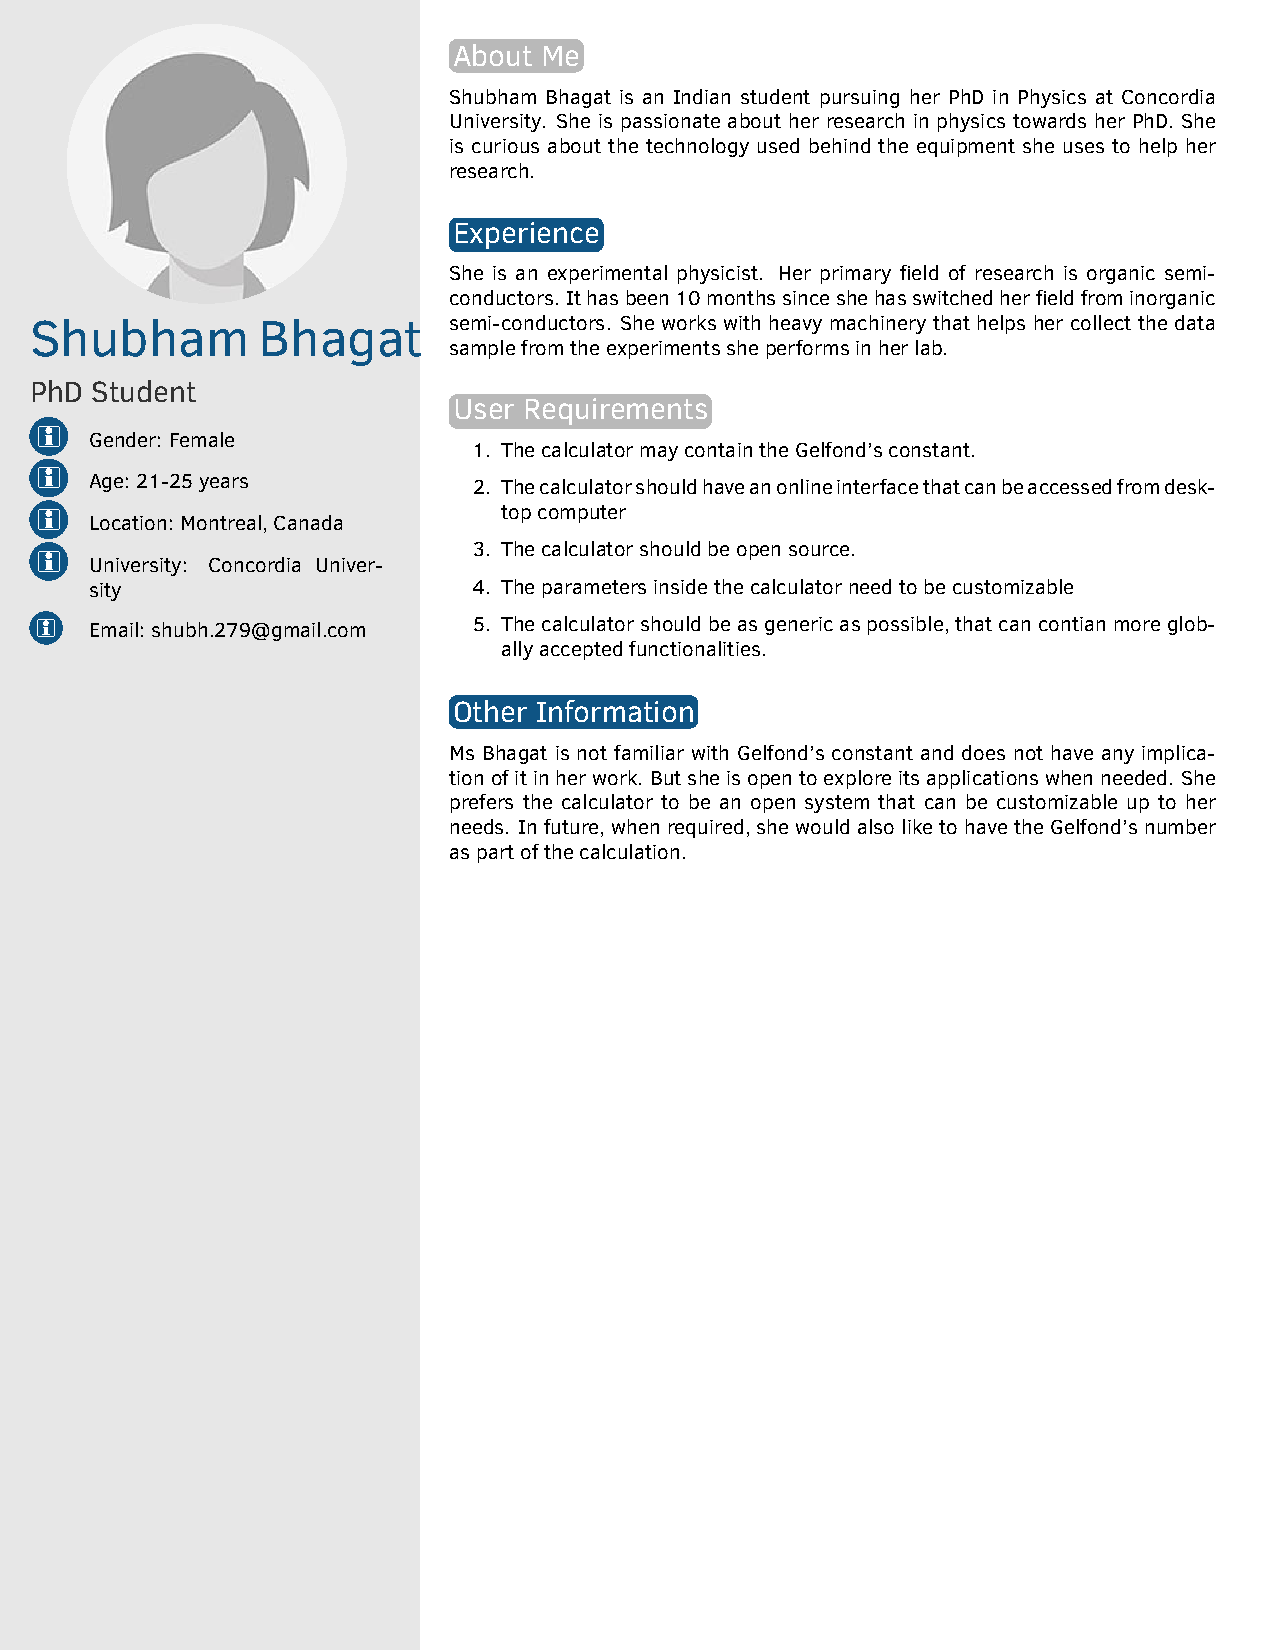
\includepdf[scale=0.7,pages=1,pagecommand=\section{Persona}]{persona/persona.pdf}

\section{Domain Model}
\begin{center}
    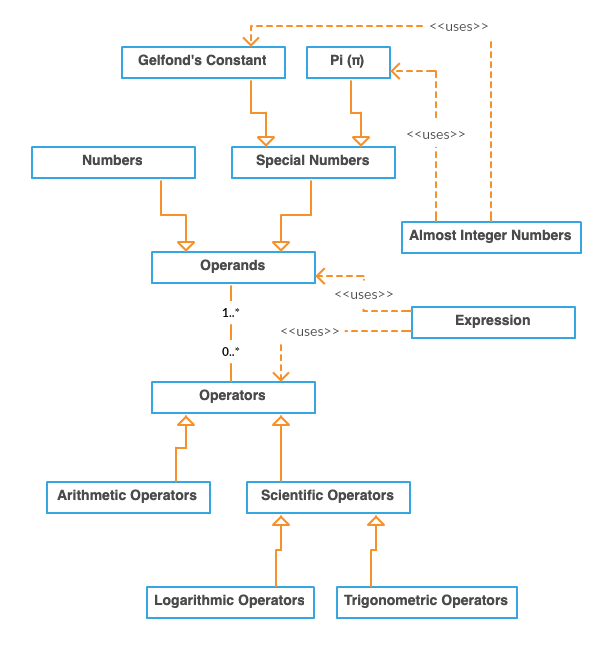
\includegraphics[scale=0.6]{images/n4-domain-model.png}
\end{center}

\clearpage

\section{Use Case Model}
\subsection{Use Cases}
\begin{center}
    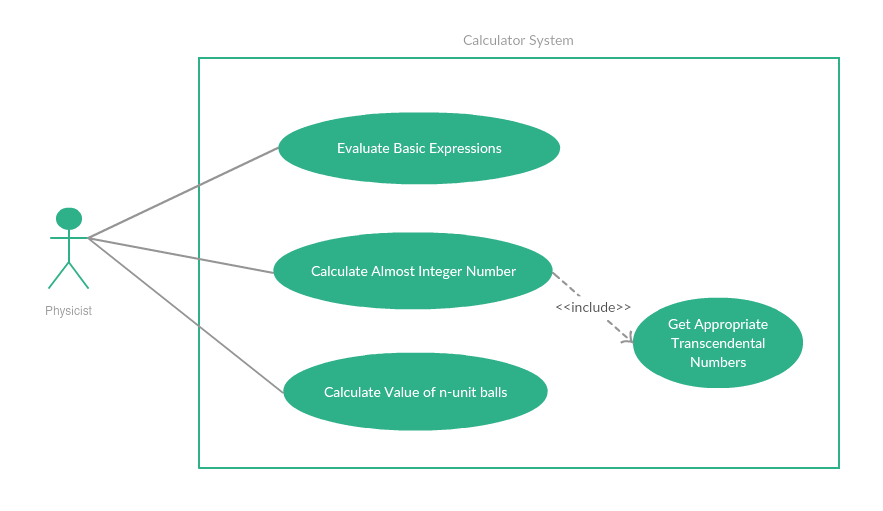
\includegraphics[scale=0.45]{images/n4-use-case.png}
\end{center}
\begin{flushleft}
Here are the sequence diagrams for these three cases.
\end{flushleft}

\subsection{Sequence for Basic Operations}
\begin{center}
    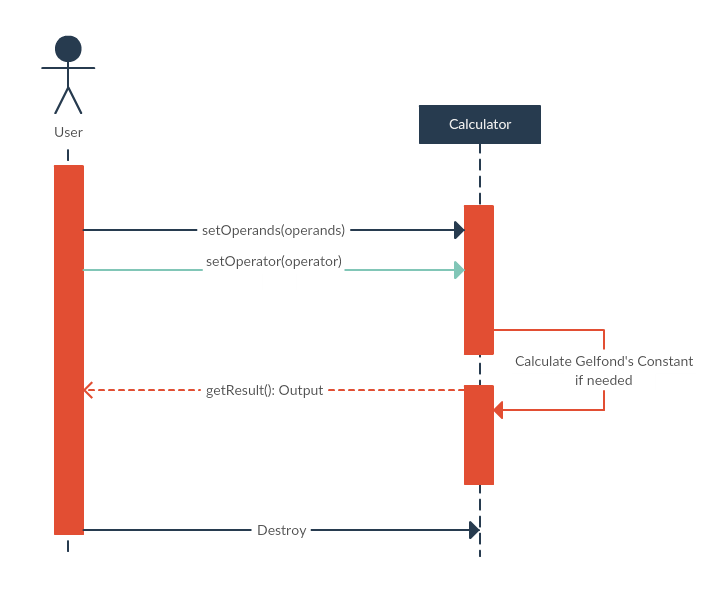
\includegraphics[scale=0.38]{images/n4-sequence-0.png}    
\end{center}

\subsection{Sequence for Almost Integer Numbers}
\begin{center}
    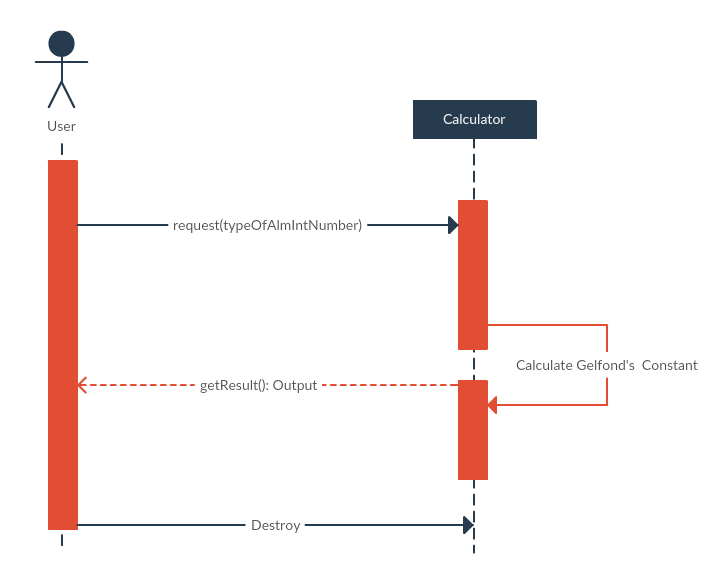
\includegraphics[scale=0.4]{images/n4-sequence-1.png}
\end{center}

\subsection{Sequence for n-ball}
\begin{center}
    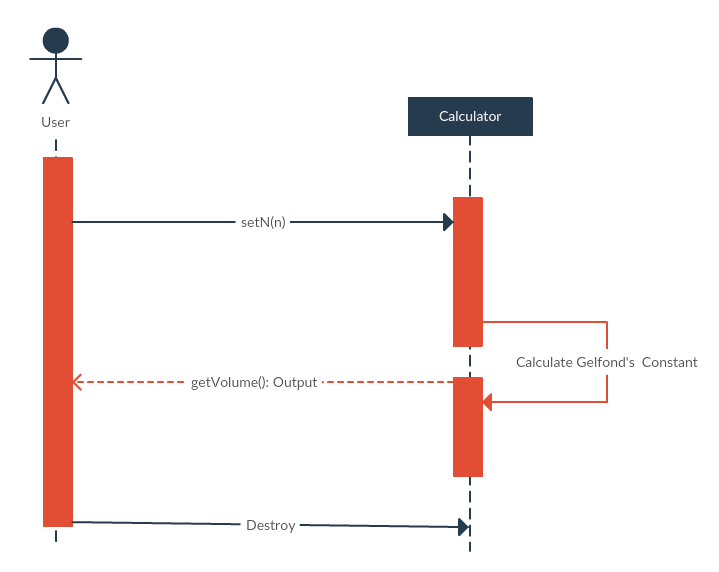
\includegraphics[scale=0.4]{images/n4-sequence-2.png}
\end{center}

\subsection{Sequence for }

\subsection{Activity Model}
\begin{center}
    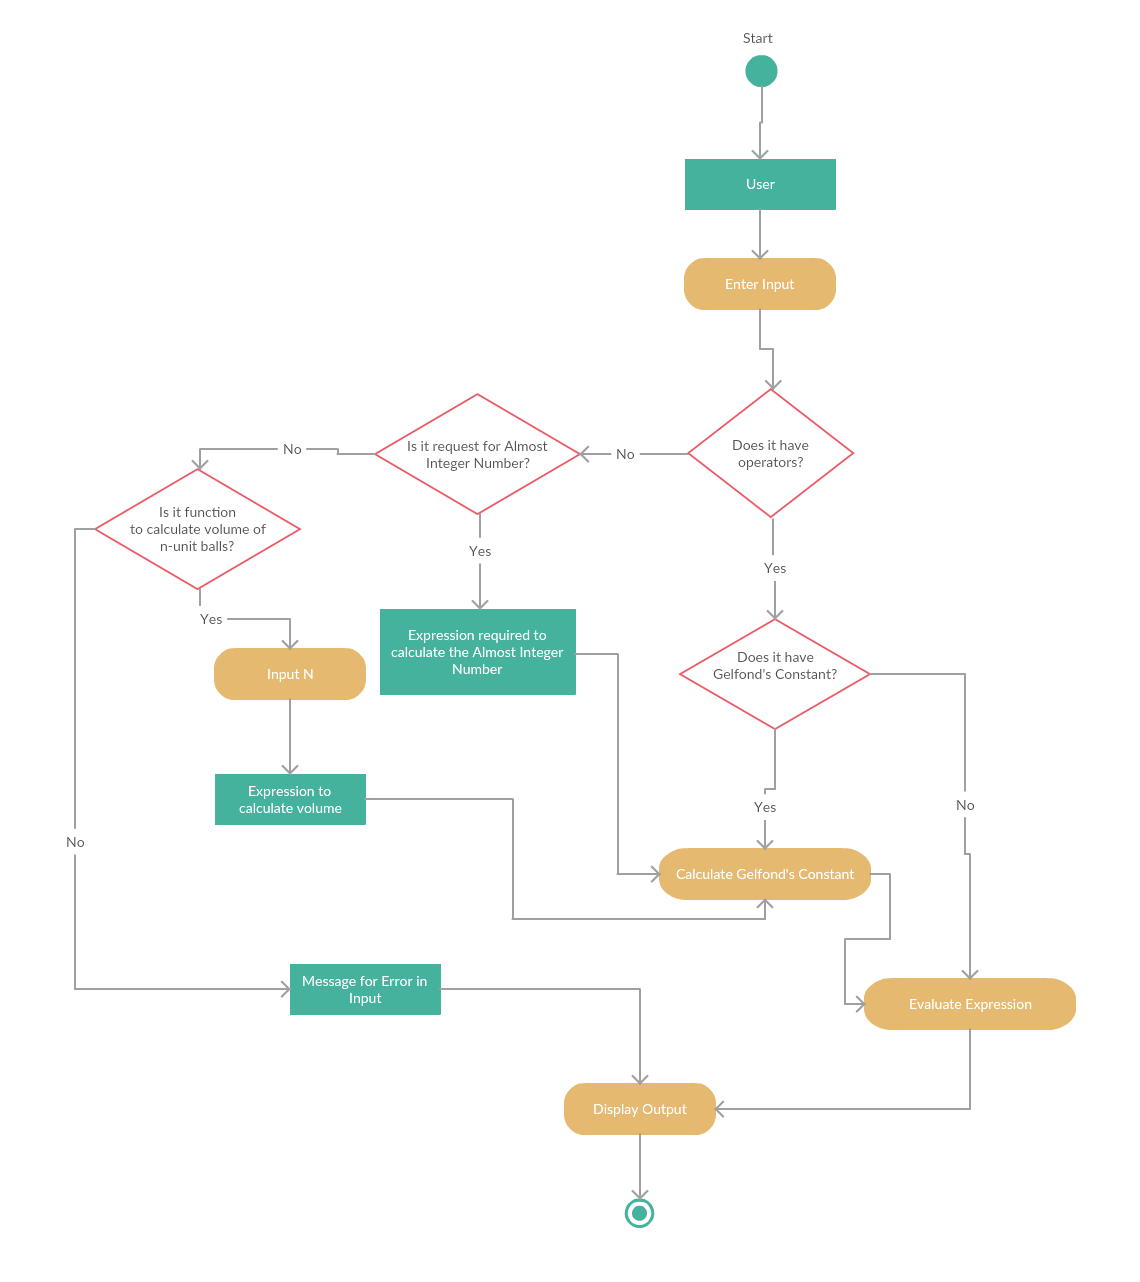
\includegraphics[scale=0.37]{images/n4-activity-model.png}
\end{center}

\printbibliography
\end{document}
